\chapter{Customization}

Some customization options are available for InVesalius users. They are shown as follow.

\section{Tools menu}

To hide/show the side tools menu, click the button shown in figure
\ref{fig:layout_full_original}.

\begin{figure}[!htb]
\centering

\includegraphics[scale=0.5]{layout_full_original}
\caption{Shortcut to hide/show side tools menu}
\label{fig:layout_full_original}
\end{figure}

With the menu hidden, the image visualization area in InVeslaius is expanded, as illustrated in figure \ref{fig:closed_tool_menu}.

\begin{figure}[!htb]
\centering
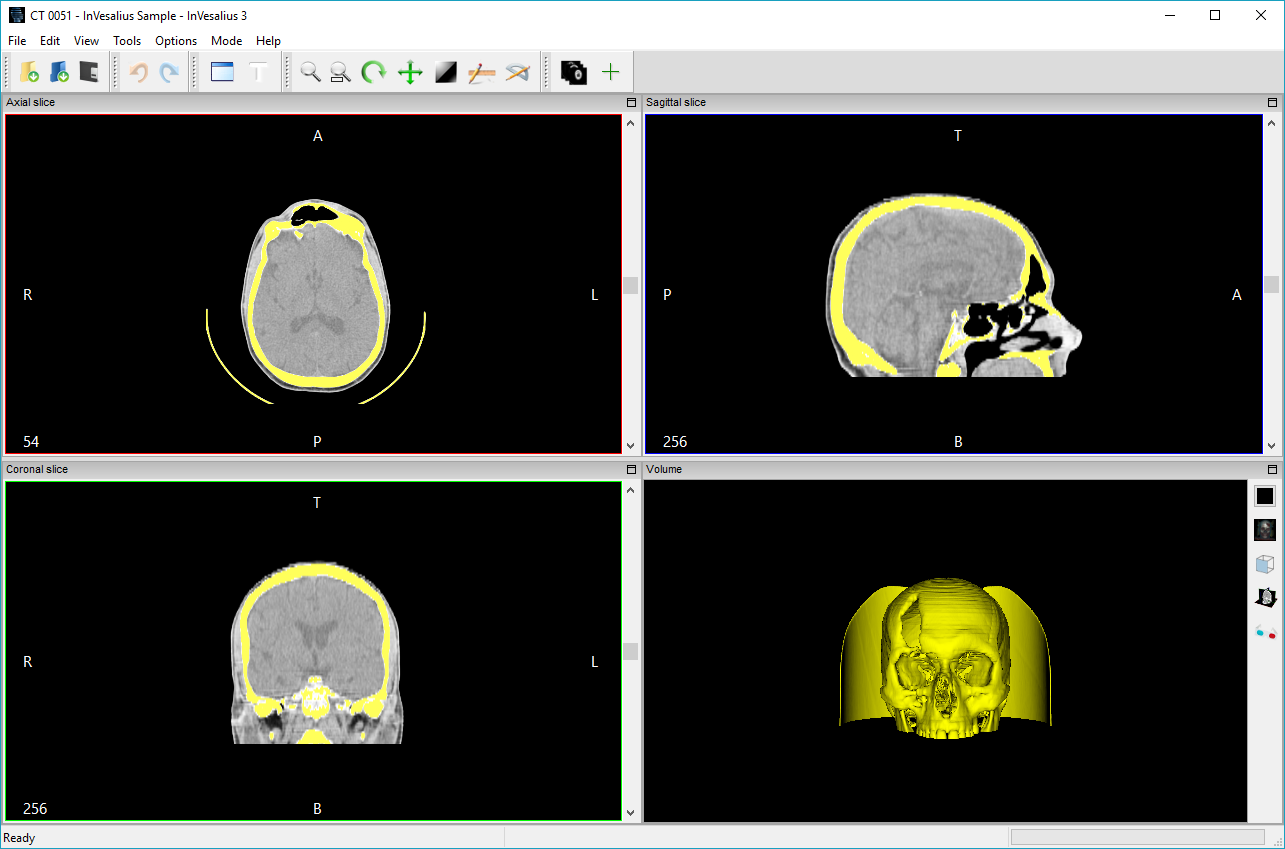
\includegraphics[scale=0.4]{window_mpr_not_painels_en.png}
\caption{Side menu hidden}
\label{fig:closed_tool_menu}
\end{figure}

\newpage

\section{Automatic positioning of volume/surface}

To automatic set the visualization position of a volume or surface,
click on the icon shown in figure \ref{fig:3d_automatic_position}
(located in the inferior right corner of InVesalius screen) and choose one of the available options for visualization.

\begin{figure}[!htb]
\centering
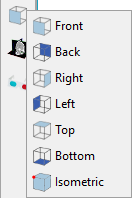
\includegraphics[scale=0.45]{3d_automatic_position_en.png}
\caption{Options for visualization positioning}
\label{fig:3d_automatic_position}
\end{figure}

\section{Background color of volume/surface window}

To change the background color of volume/surface window, click on the shortcut shown in figure
\ref{fig:button_select_color_2}. The shortcut is also located in the inferior right cornen of InVesalius screen.

\begin{figure}[!htb]
\centering
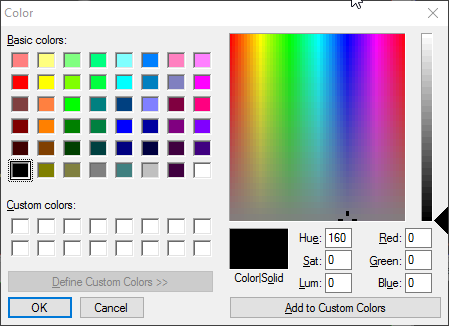
\includegraphics[scale=0.8]{colour_button_en.png}
\caption{Shortcut to background color of volume/surface window}
\label{fig:button_select_color_2}
\end{figure}

A window for color selection opens, as in figure \ref{fig:color_window_background}.
Next, just click over the desired color and then click \textbf{OK}.

\begin{figure}[!htb]
\centering
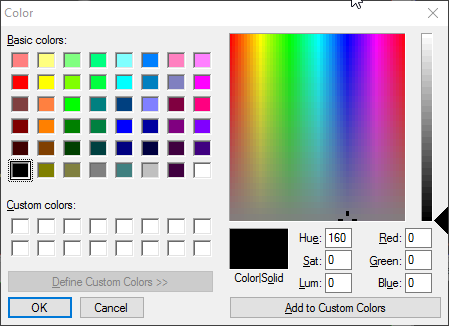
\includegraphics[scale=0.6]{surface_select_color_windows_so_en.png}
\caption{Background color selection}
\label{fig:color_window_background}
\end{figure}

The figure \ref{fig:background_color} illustrates the correspondent window with modified background color.

\begin{figure}[!htb]
\centering
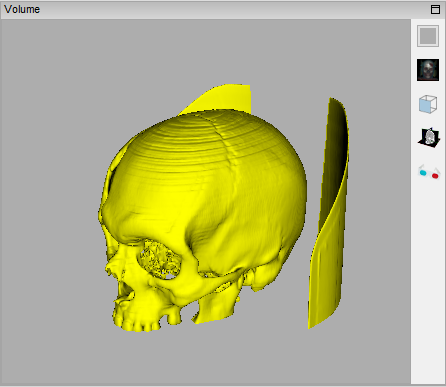
\includegraphics[scale=0.7]{3d_background_changed.png}
\caption{Background color modified}
\label{fig:background_color}
\end{figure}

\newpage

\section{Show/hide text in 2D windows}

To show or hide the texts in 2D image windows, click in the shortcut illustrated
in figure \ref{fig:text}, located in tools bar.

\begin{figure}[!htb]
\centering

\includegraphics[scale=0.7]{text}
\caption{Shorcut to show or hide texts}
\label{fig:text}
\end{figure}

Figures \ref{fig:text_on} and \ref{fig:text_off} exhibit texts enabled and disabled, respectively.

\begin{figure}[!htb]
\centering
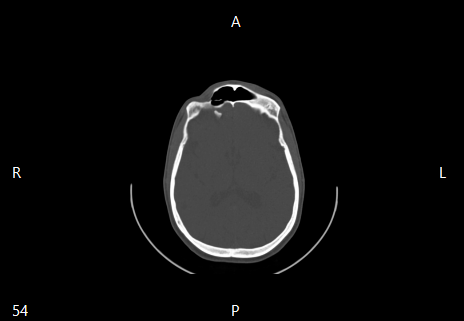
\includegraphics[scale=0.5]{axial_en.png}
\caption{Show texts enabled}
\label{fig:text_on}
\end{figure}

\begin{figure}[!htb]
\centering
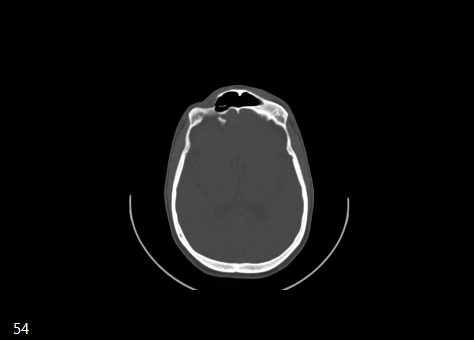
\includegraphics[scale=0.5]{axial_no_tex_en.png}
\caption{Show texts disabled}
\label{fig:text_off}
\end{figure}
